%!TEX TS-program = Arara
% arara: pdflatex: {shell: yes}
% arara: pdflatex: {shell: yes}
\documentclass[12pt,ngerman,parskip=half]{scrreprt}

\usepackage[utf8]{inputenc}
\usepackage[T1]{fontenc}
\usepackage{booktabs}
\usepackage{babel}
\usepackage{graphicx}
\usepackage{csquotes}
\usepackage{paralist}
\usepackage{xcolor}
\usepackage{blindtext}
\usepackage{hyperref}
\usepackage{microtype}
\usepackage{subcaption}

\setcapindent{2em} % kein Abstand bei mehrzeiligen Captions

\author{Donald Duck}
\title{Meine Dissertation}
\date{Entenhausen, den 17.05.2022}

\includeonly{Kapitel-02,Kapitel-03}

\begin{document}
\maketitle

\tableofcontents

\listoffigures

\listoftables

\chapter{Bilder einfügen}

\blindtext

\begin{figure}[hbtp!]%\centering%
\begin{center}
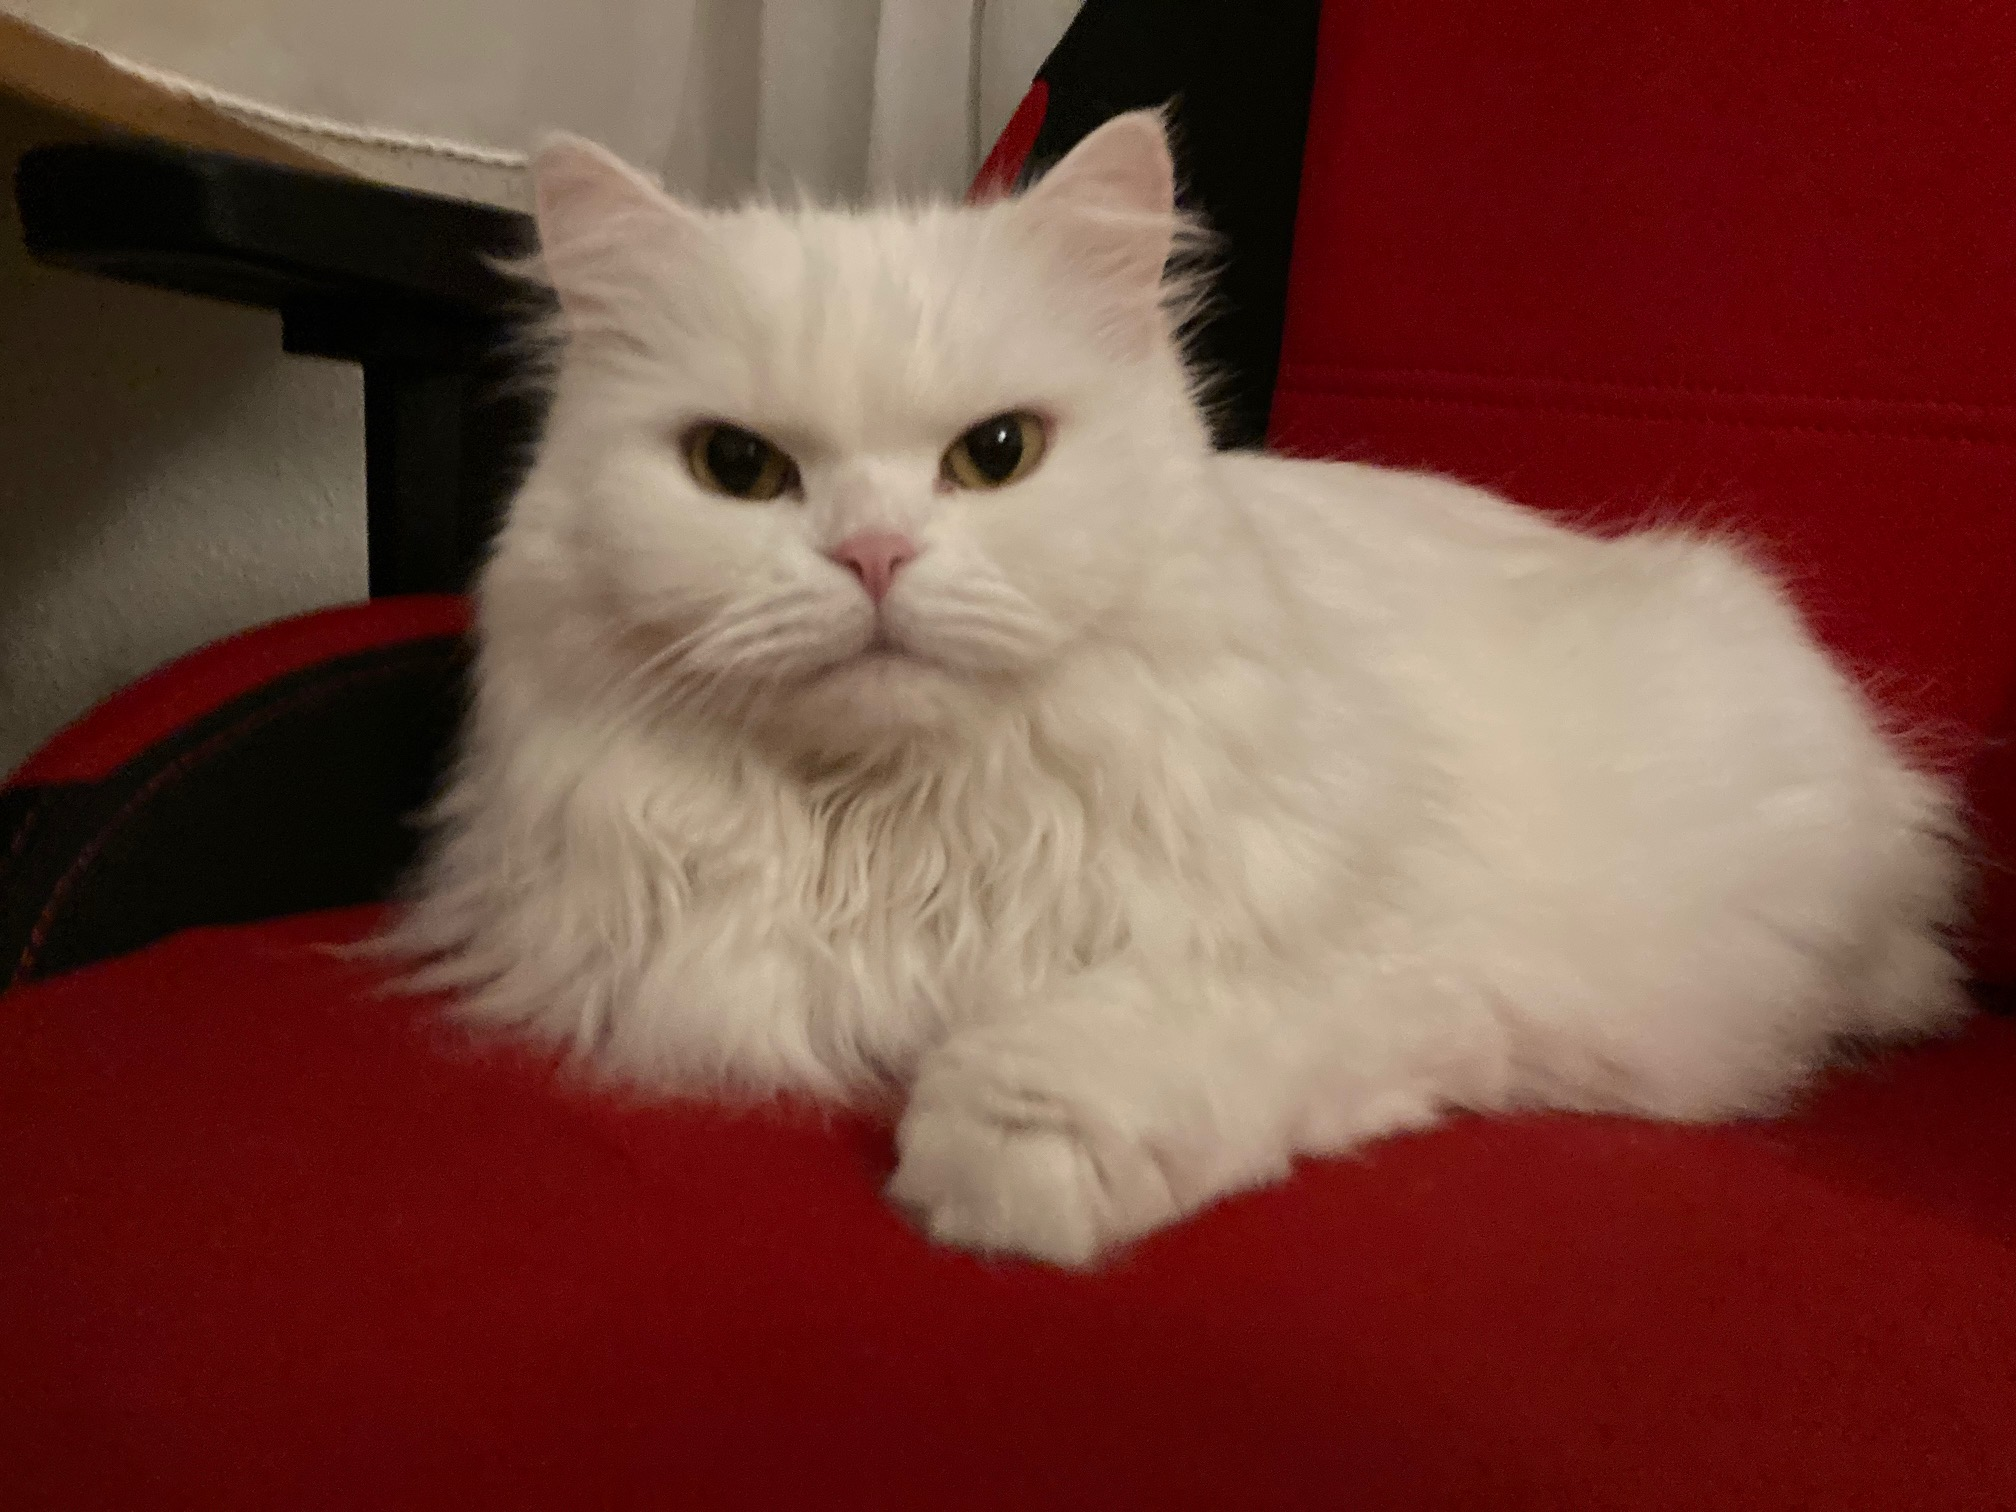
\includegraphics[width=0.9\textwidth]{Bilder/Katze}
\end{center}
\caption{Meine Katze, \blindtext}
\end{figure}
% h = here, t = top, b = bottom, p = Leerseite


\blindtext

\begin{figure}
\centering
\subcaptionbox{Eine Katze \label{cat1}}
{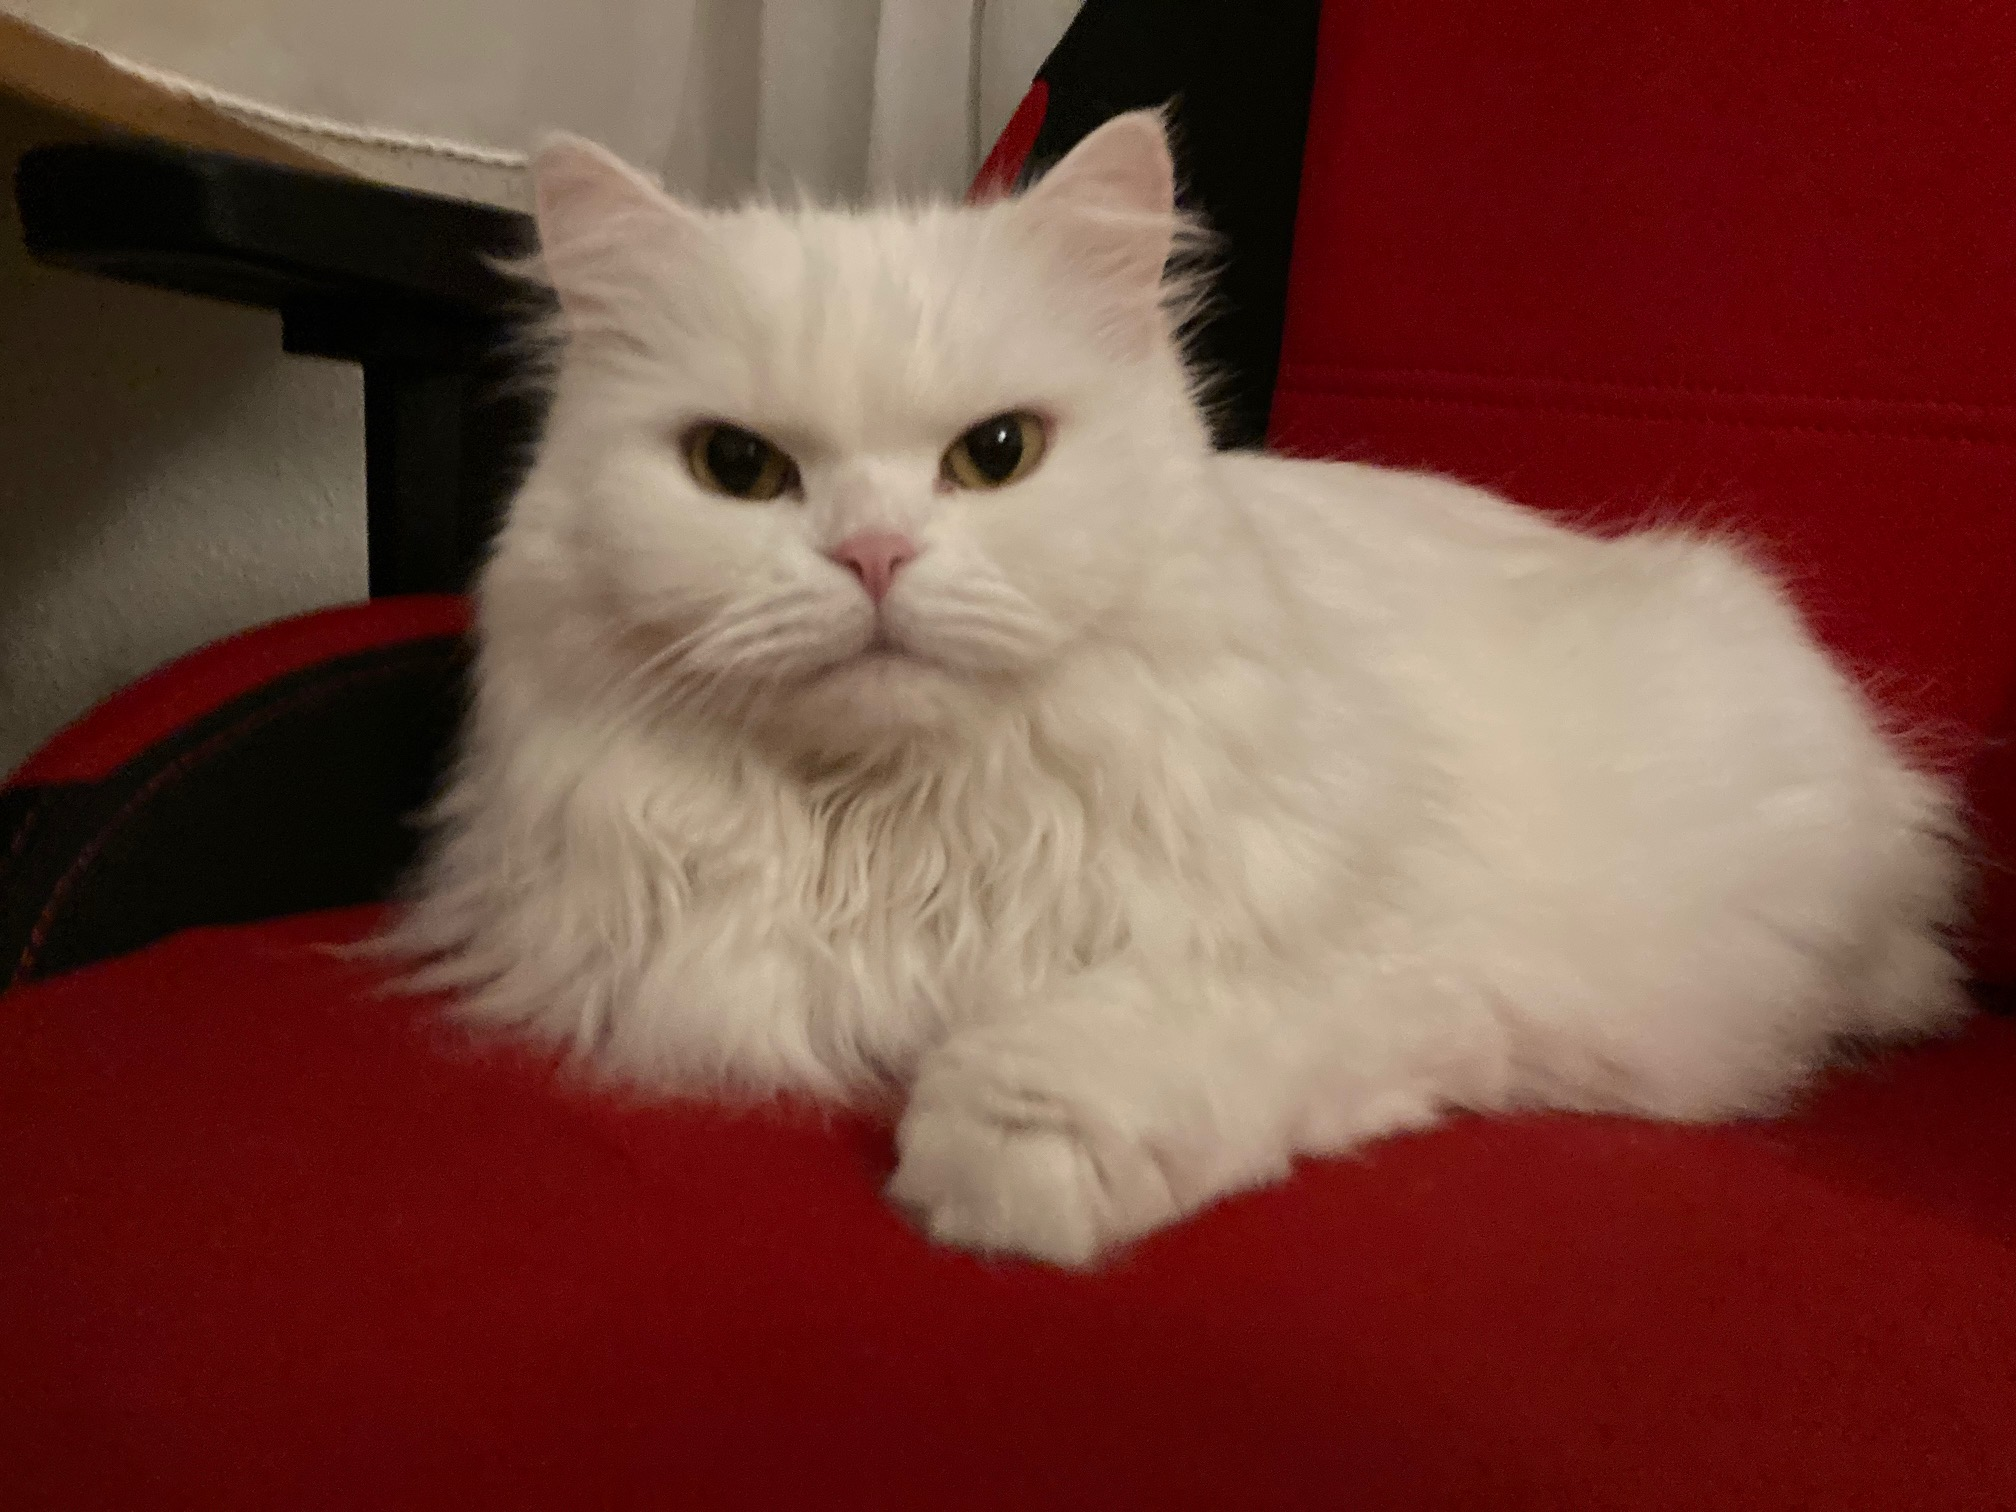
\includegraphics[width=0.49\textwidth]{Bilder/Katze}}
\subcaptionbox{Die selbe Katze \label{cat2}}
{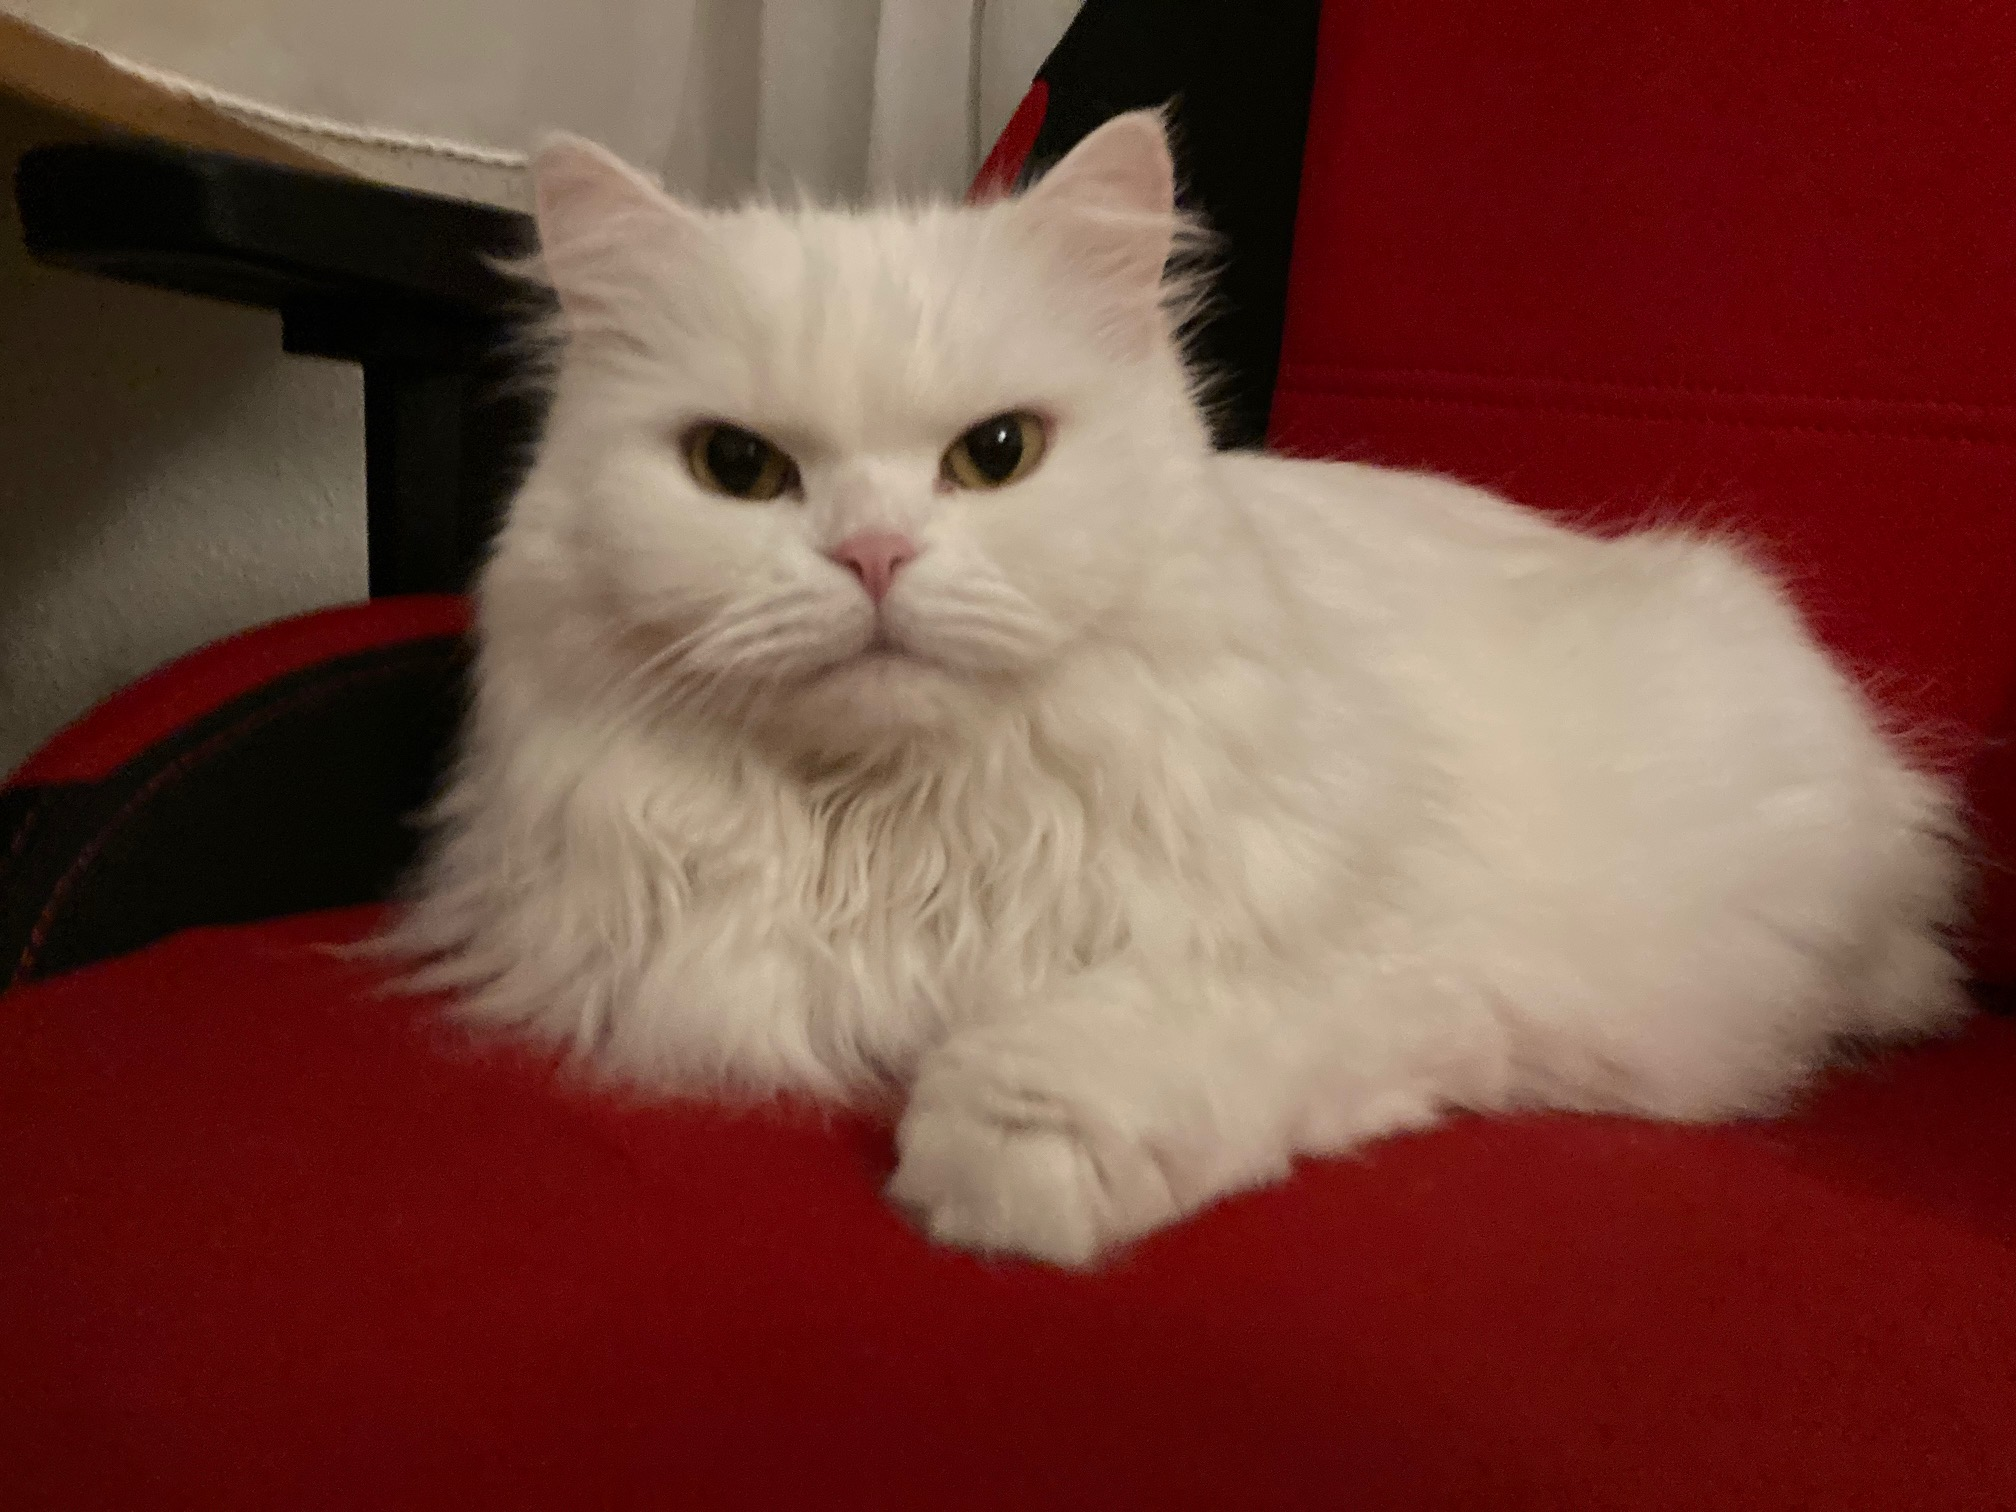
\includegraphics[width=0.49\textwidth]{Bilder/Katze}}
%\caption{Zwei Katzenbilder}\label{katzenbilder}
\subcaptionbox{Eine Katze \label{cat3}}
{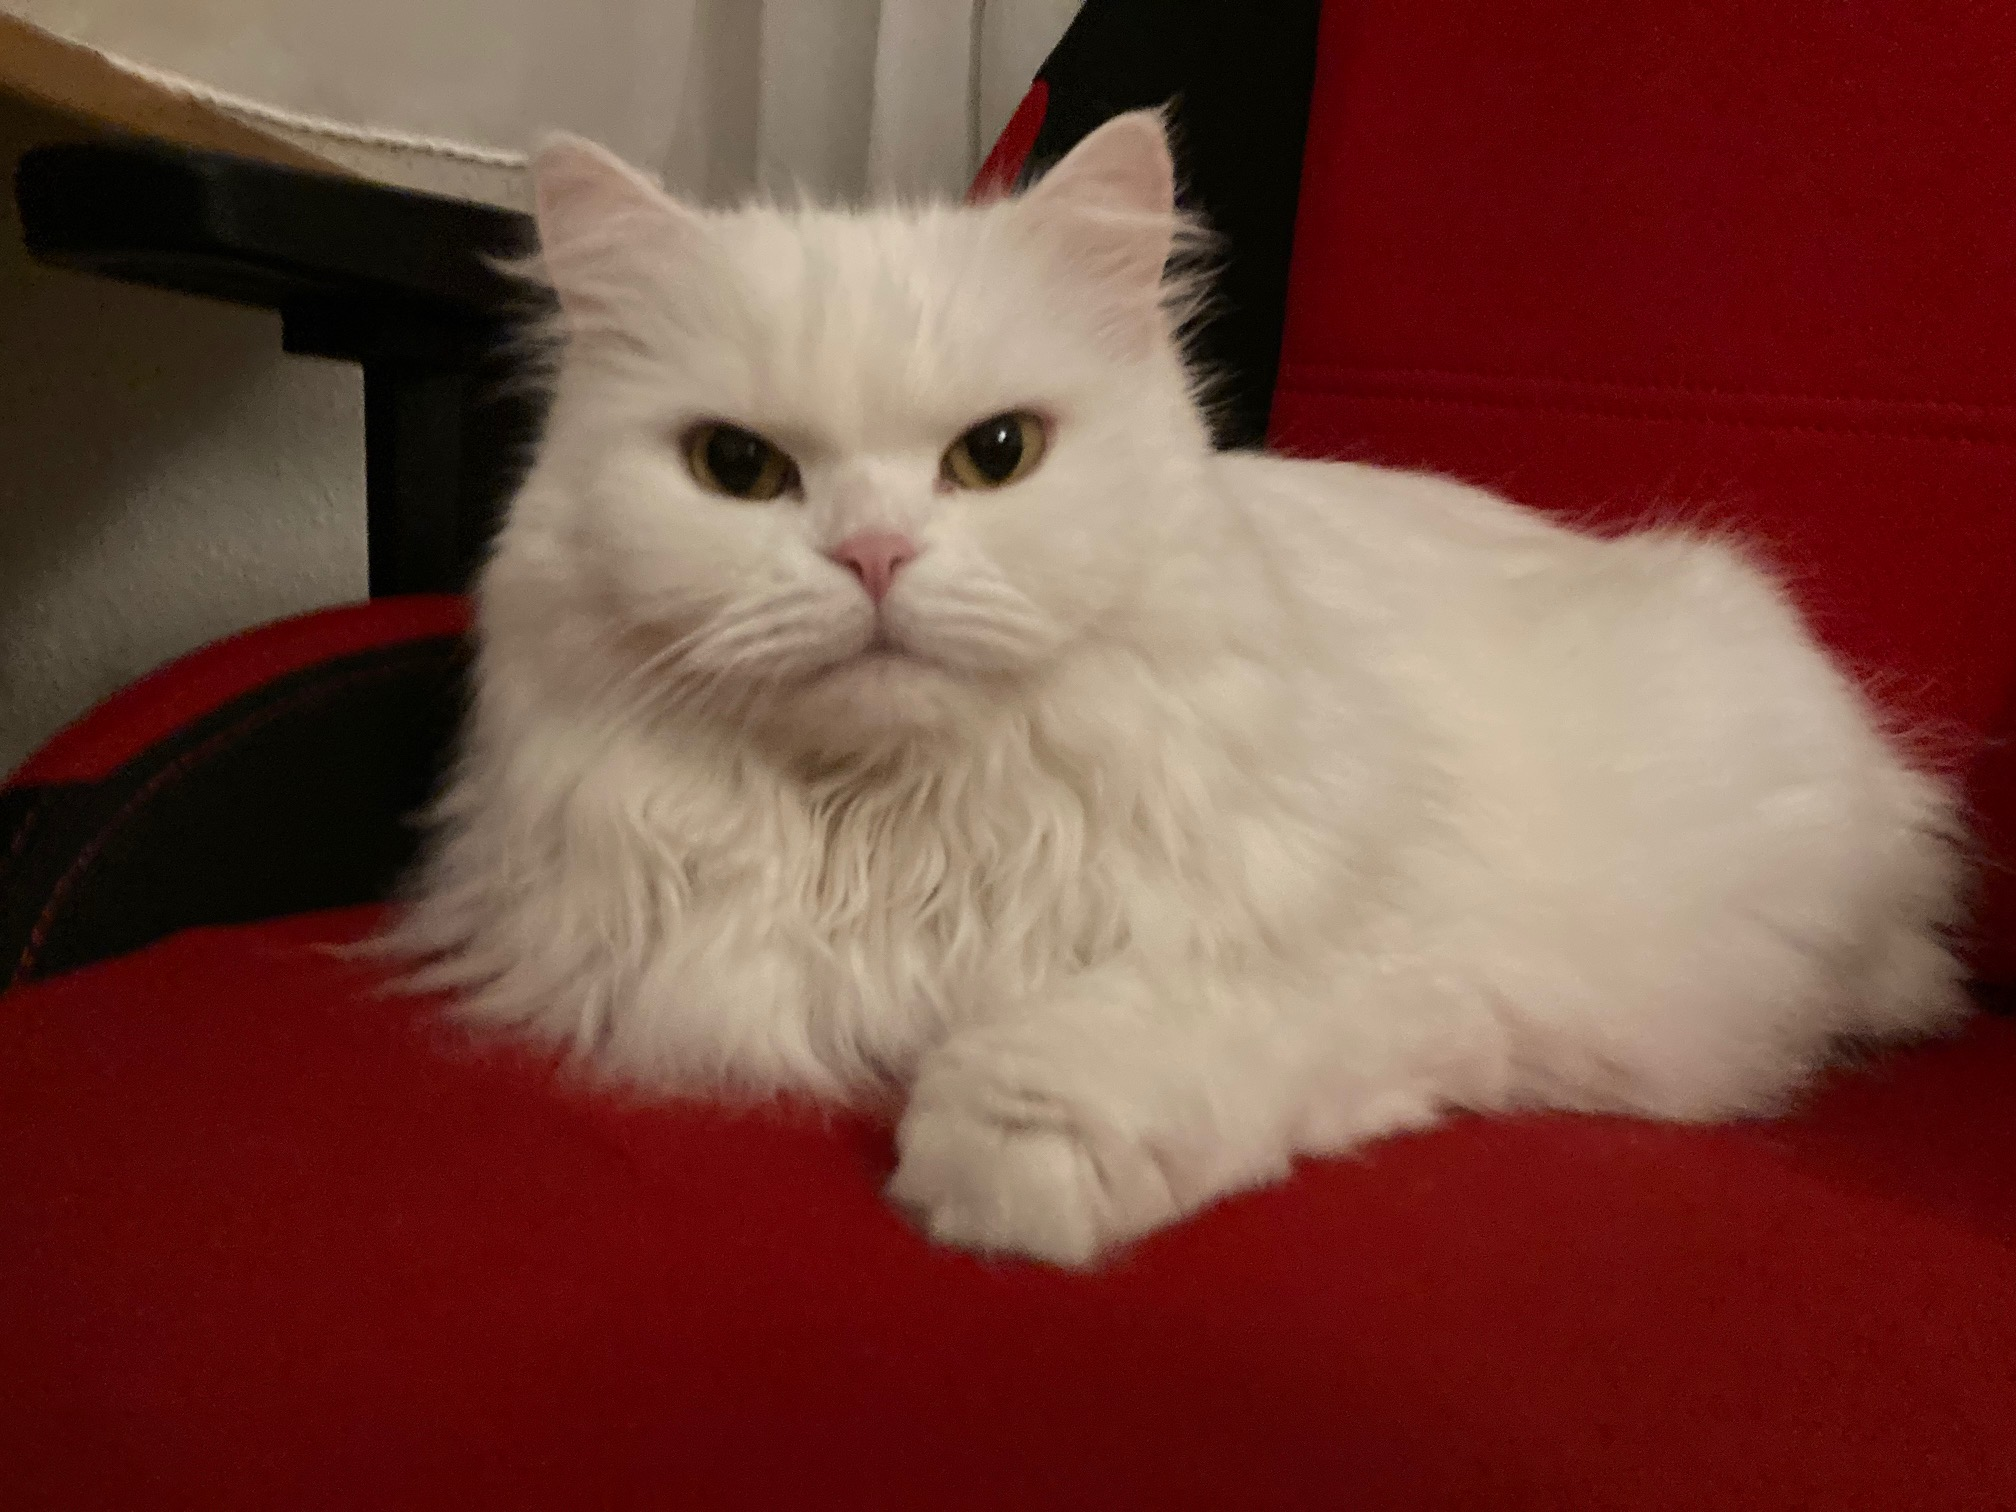
\includegraphics[width=0.49\textwidth]{Bilder/Katze}}
\subcaptionbox{Die selbe Katze \label{cat4}}
{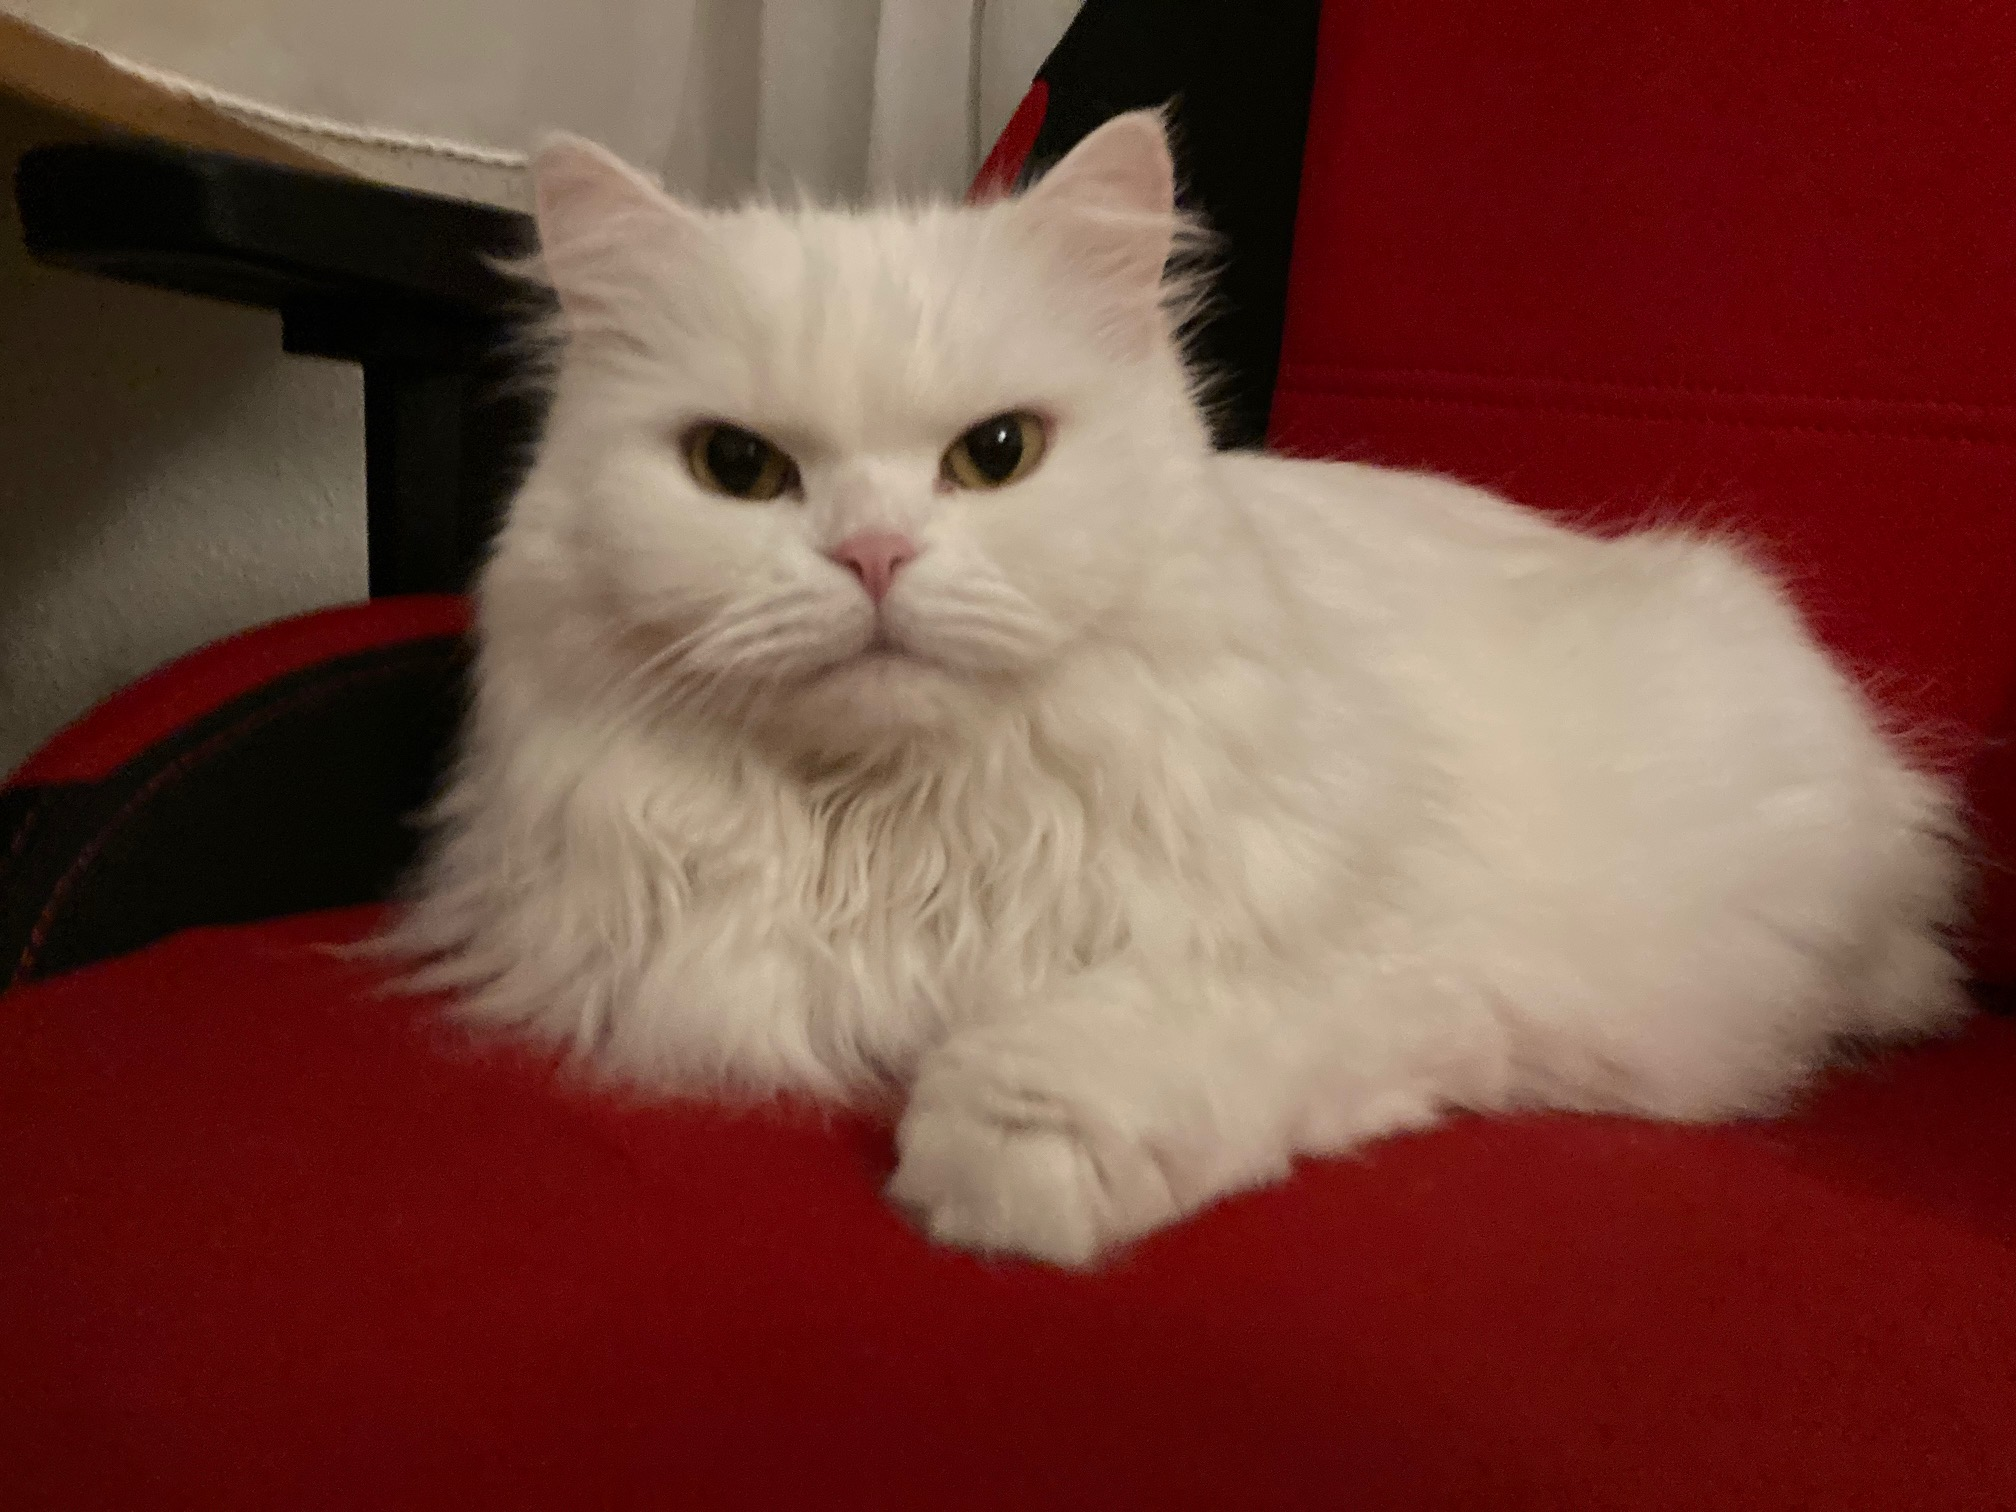
\includegraphics[width=0.49\textwidth]{Bilder/Katze}}
\caption{Zwei Katzenbilder, \blindtext[1]}\label{katzenbilder}
\end{figure}

Abbildung \ref{cat1} auf Seite \pageref{katzenbilder}

Abbildung \ref{cat2} auf Seite \pageref{katzenbilder}

Abbildung \ref{katzenbilder} auf Seite \pageref{katzenbilder}




\the\textwidth

\the\linewidth

\the\columnwidth

\begin{itemize}
	\item \the\textwidth
	\item \the\linewidth
	\item \the\columnwidth
\end{itemize}


\chapter{Bilder einfügen alternativ}

\blindtext  sdfdf dfgg sdg dfgdfgs sdfdf dfgg sdg dfgdfgs sdfdf dfgg sdg dfgdfgs sdfdf dfgg sdg dfgdfgs sdfdf dfgg sdg dfgdfgs sdfdf dfgg sdg dfgdfgs sdfdf dfgg sdg dfgdfgs sdfdf dfgg sdg dfgdfgs sdfdf dfgg sdg dfgdfgs 


\begin{minipage}{\textwidth}
\begin{center}
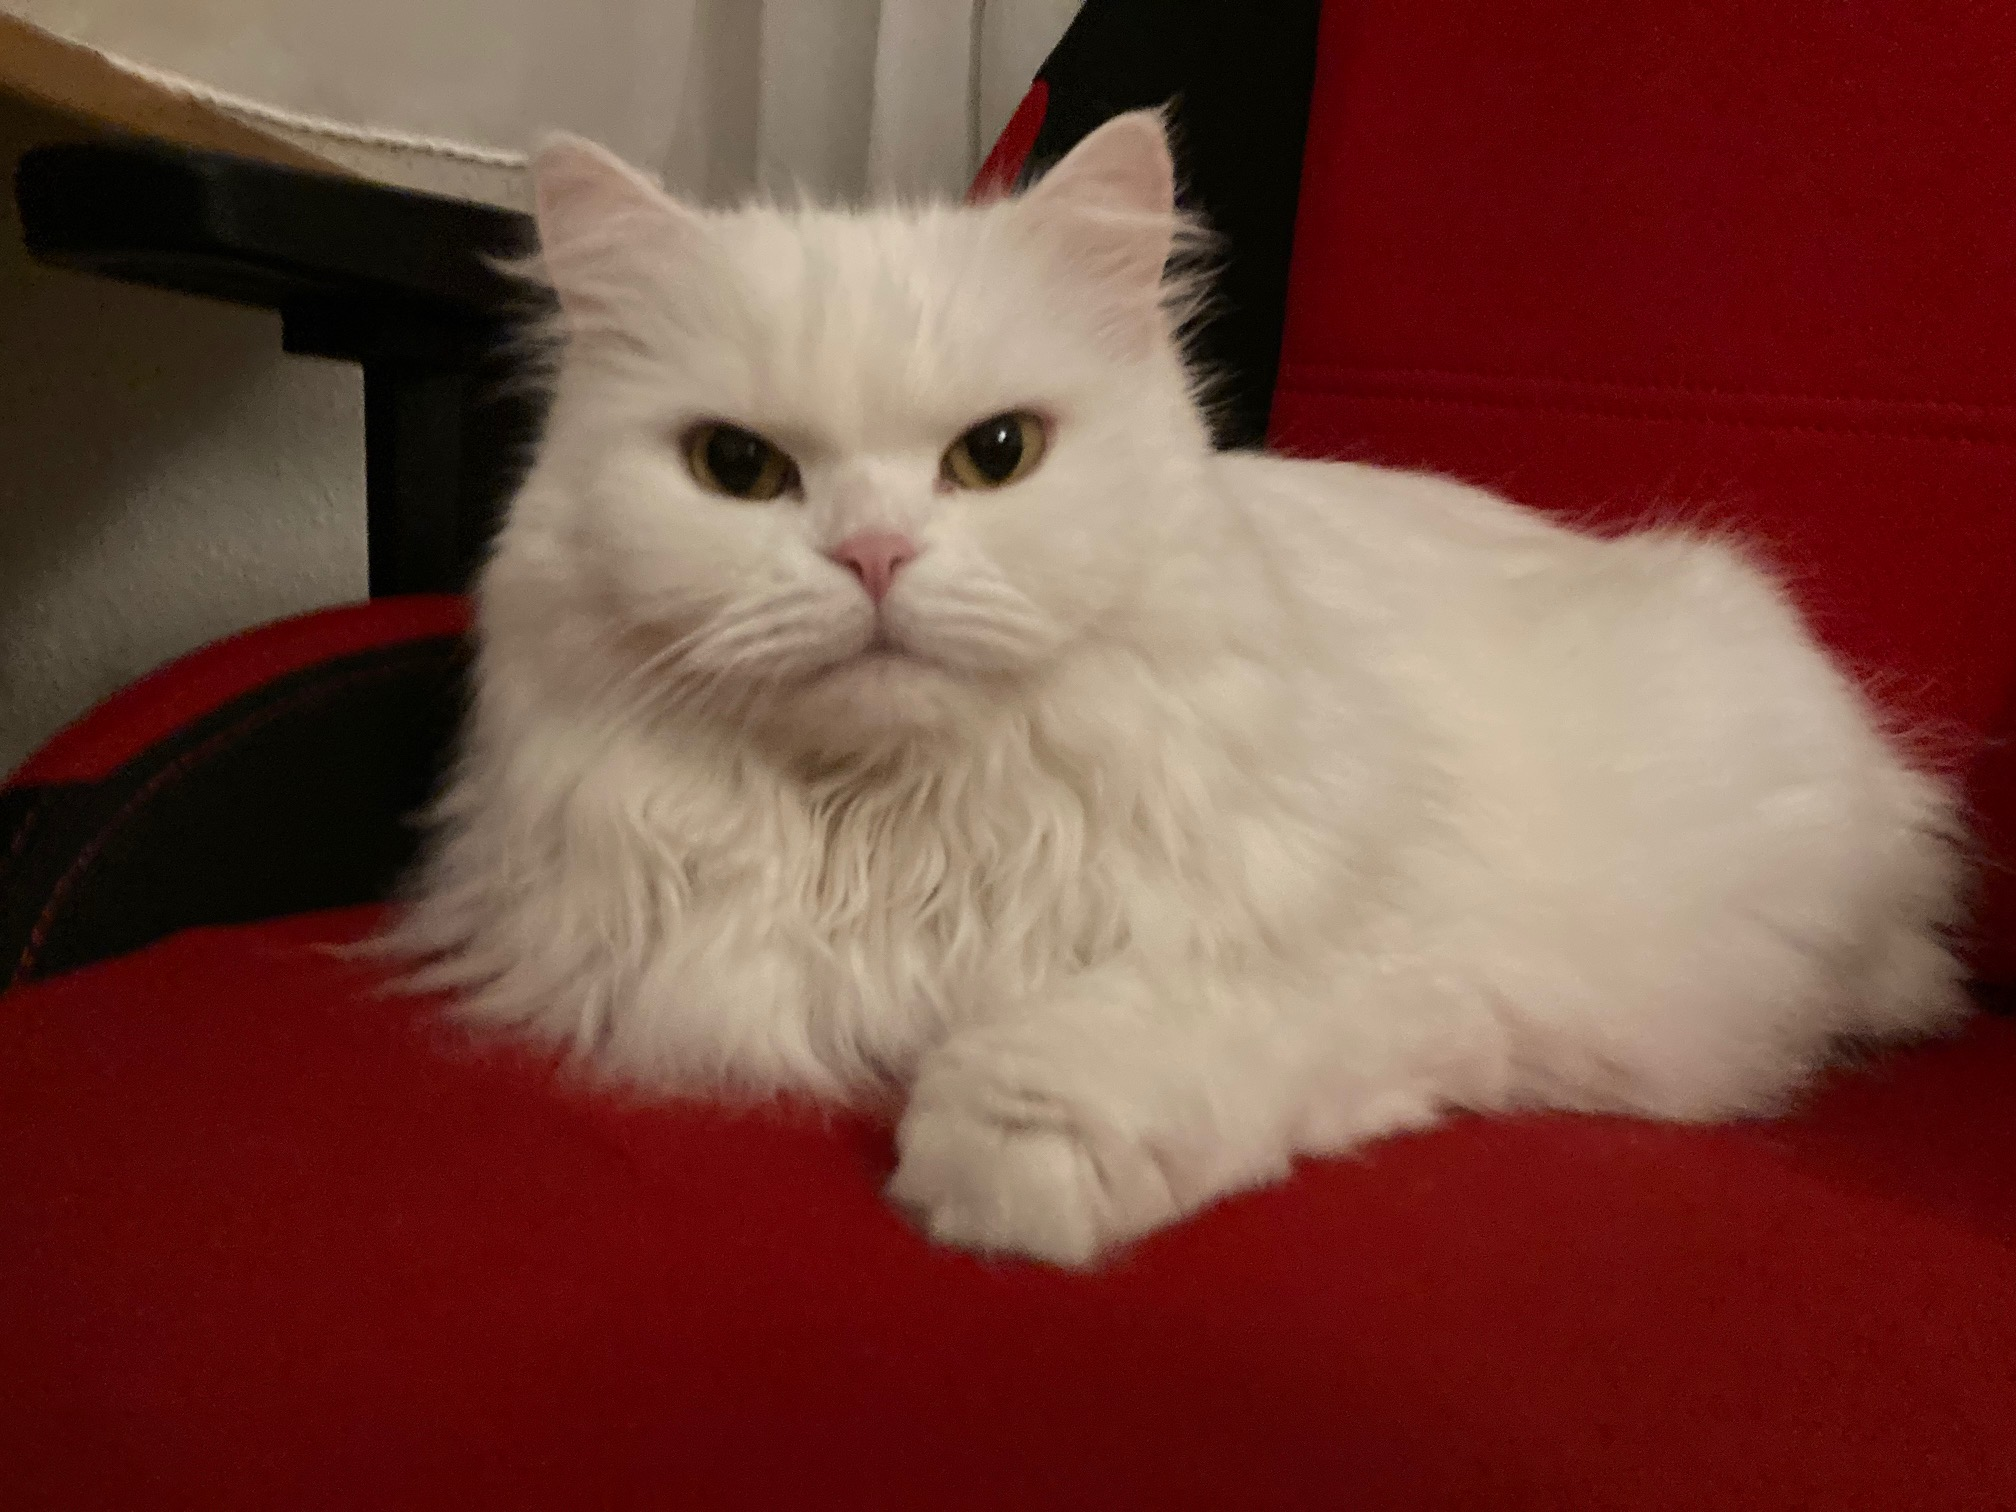
\includegraphics[width=0.9\textwidth,angle=-5]{Bilder/Katze}
\captionof{figure}{Meine Katze}
\end{center}
\end{minipage}


\blindtext


\chapter{Bilder in Tabellen}

\begin{tabular}{cc}
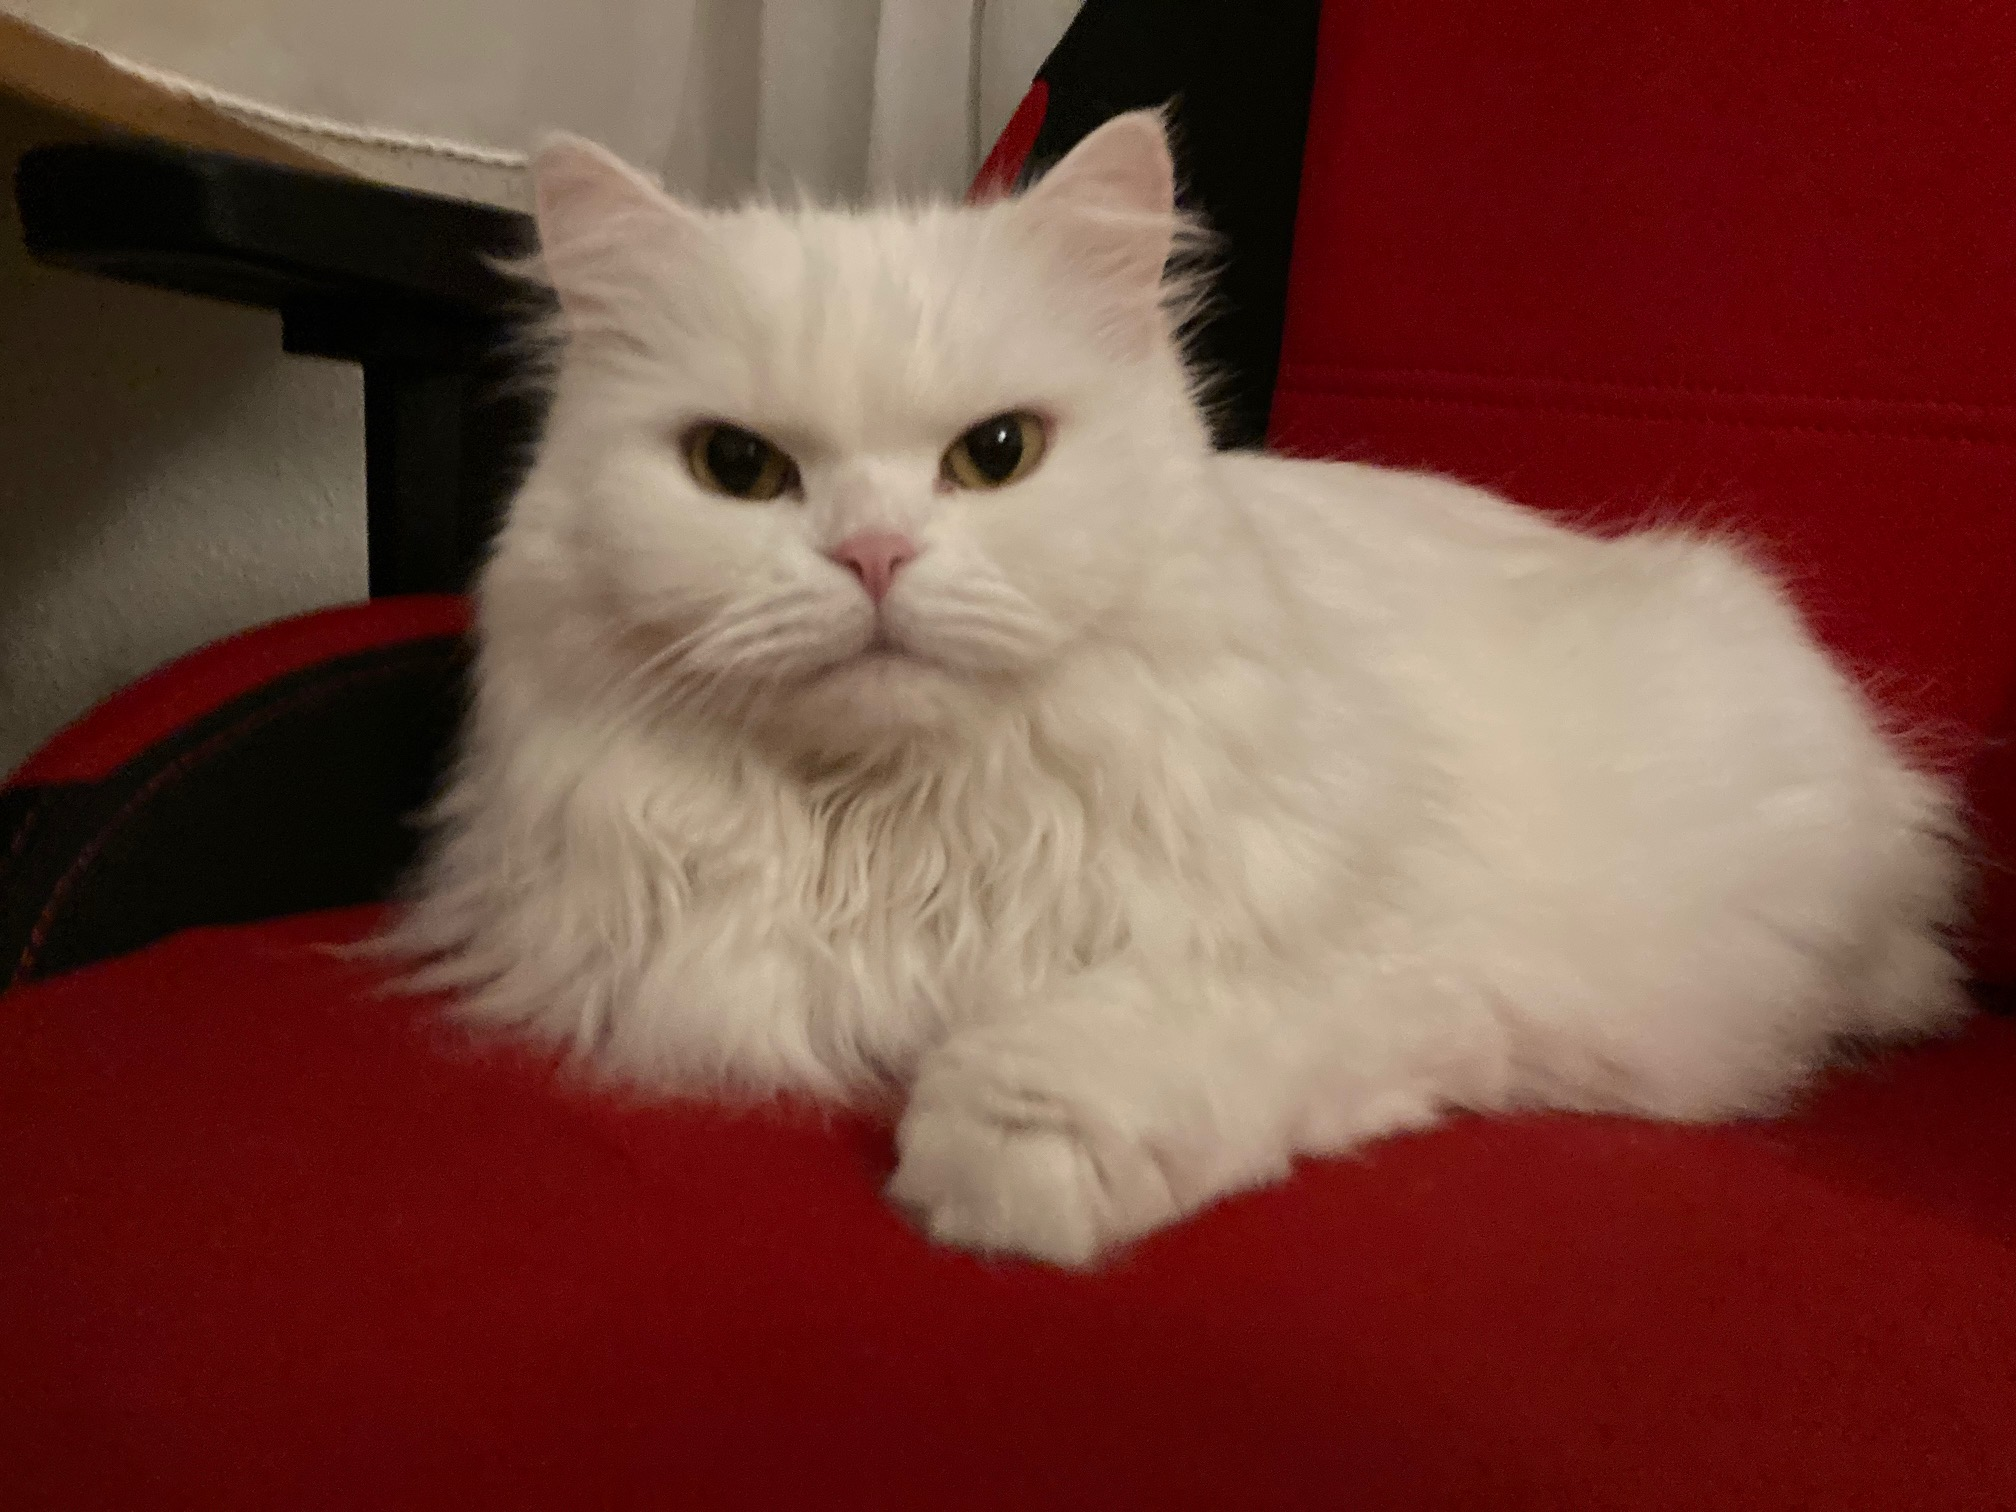
\includegraphics[width=0.45\textwidth]{Bilder/Katze} & 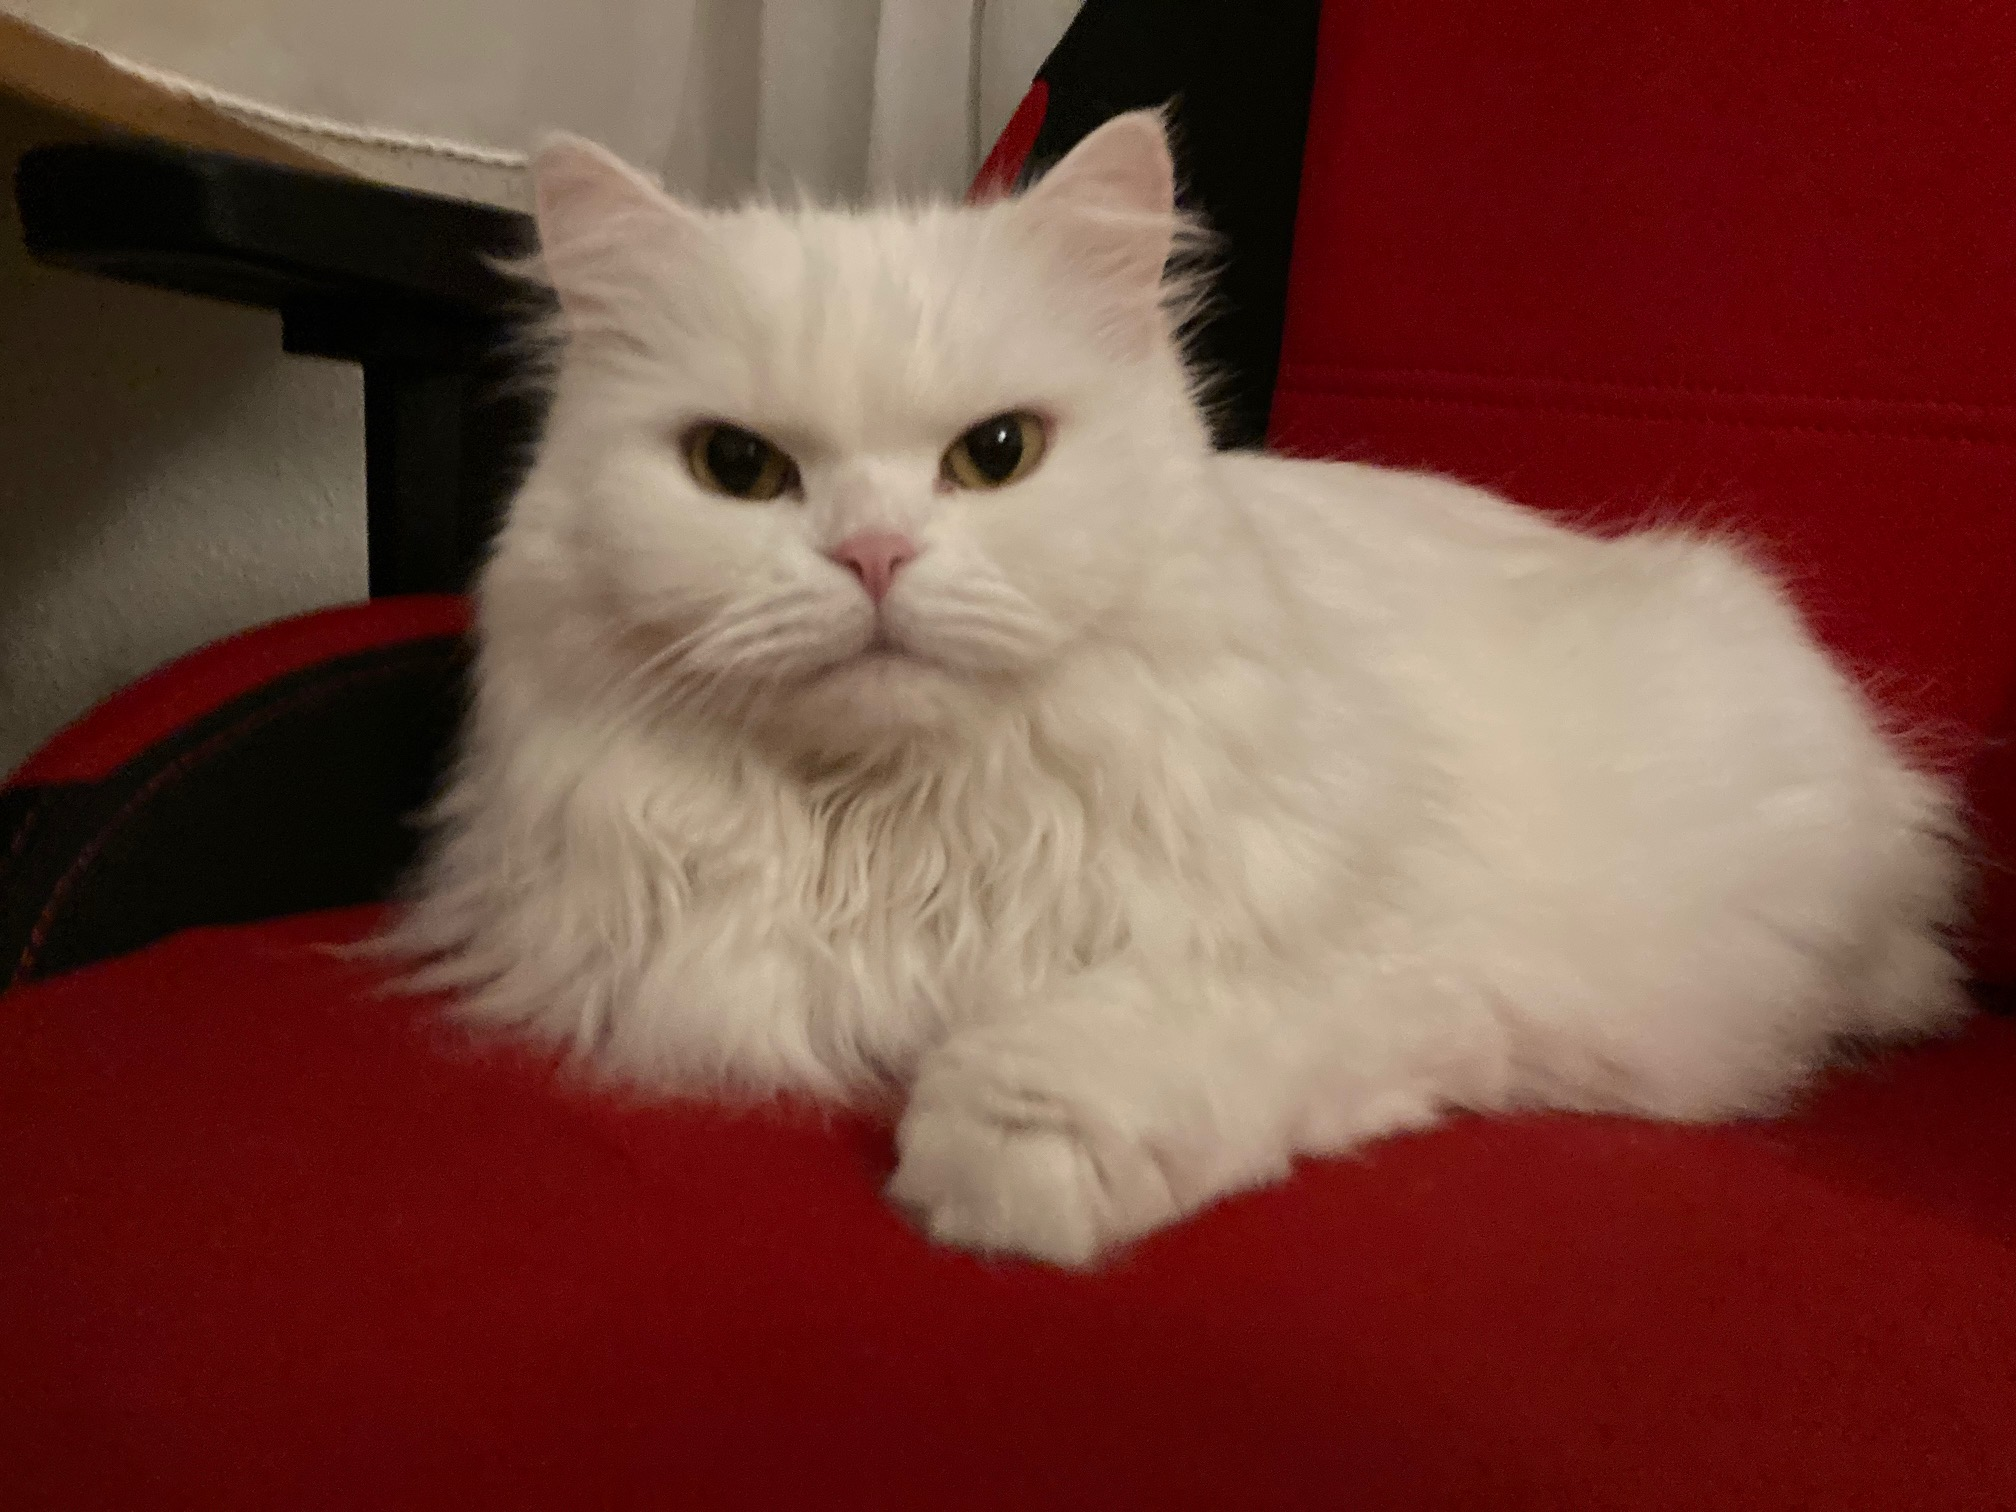
\includegraphics[height=0.4\textwidth]{Bilder/Katze} \\
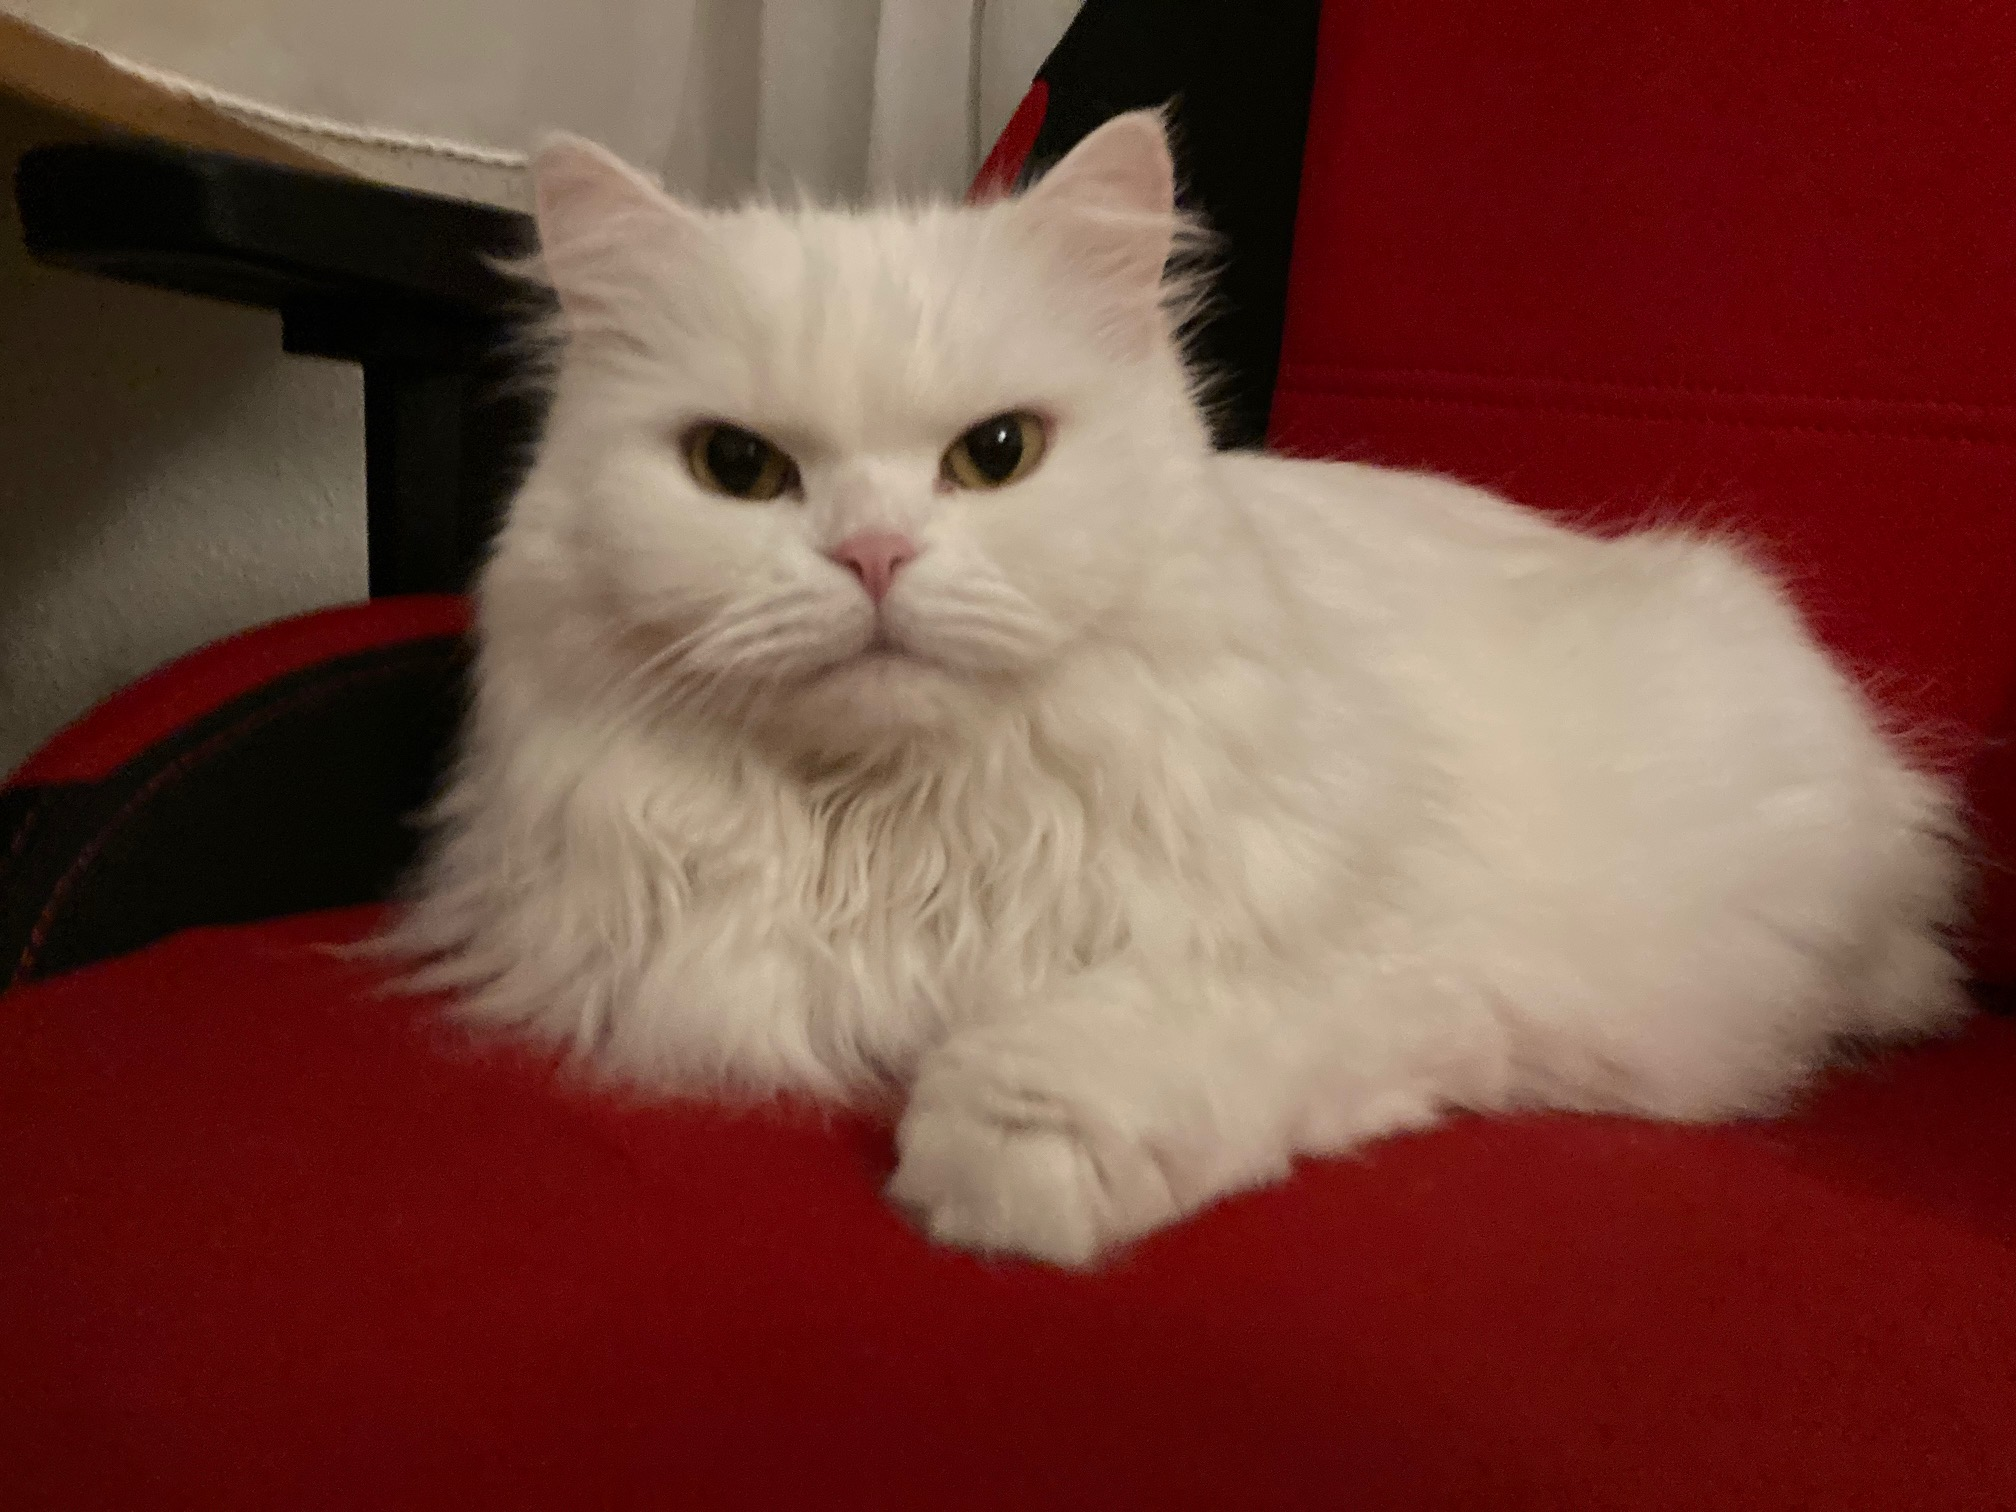
\includegraphics[width=0.49\textwidth]{Bilder/Katze} & 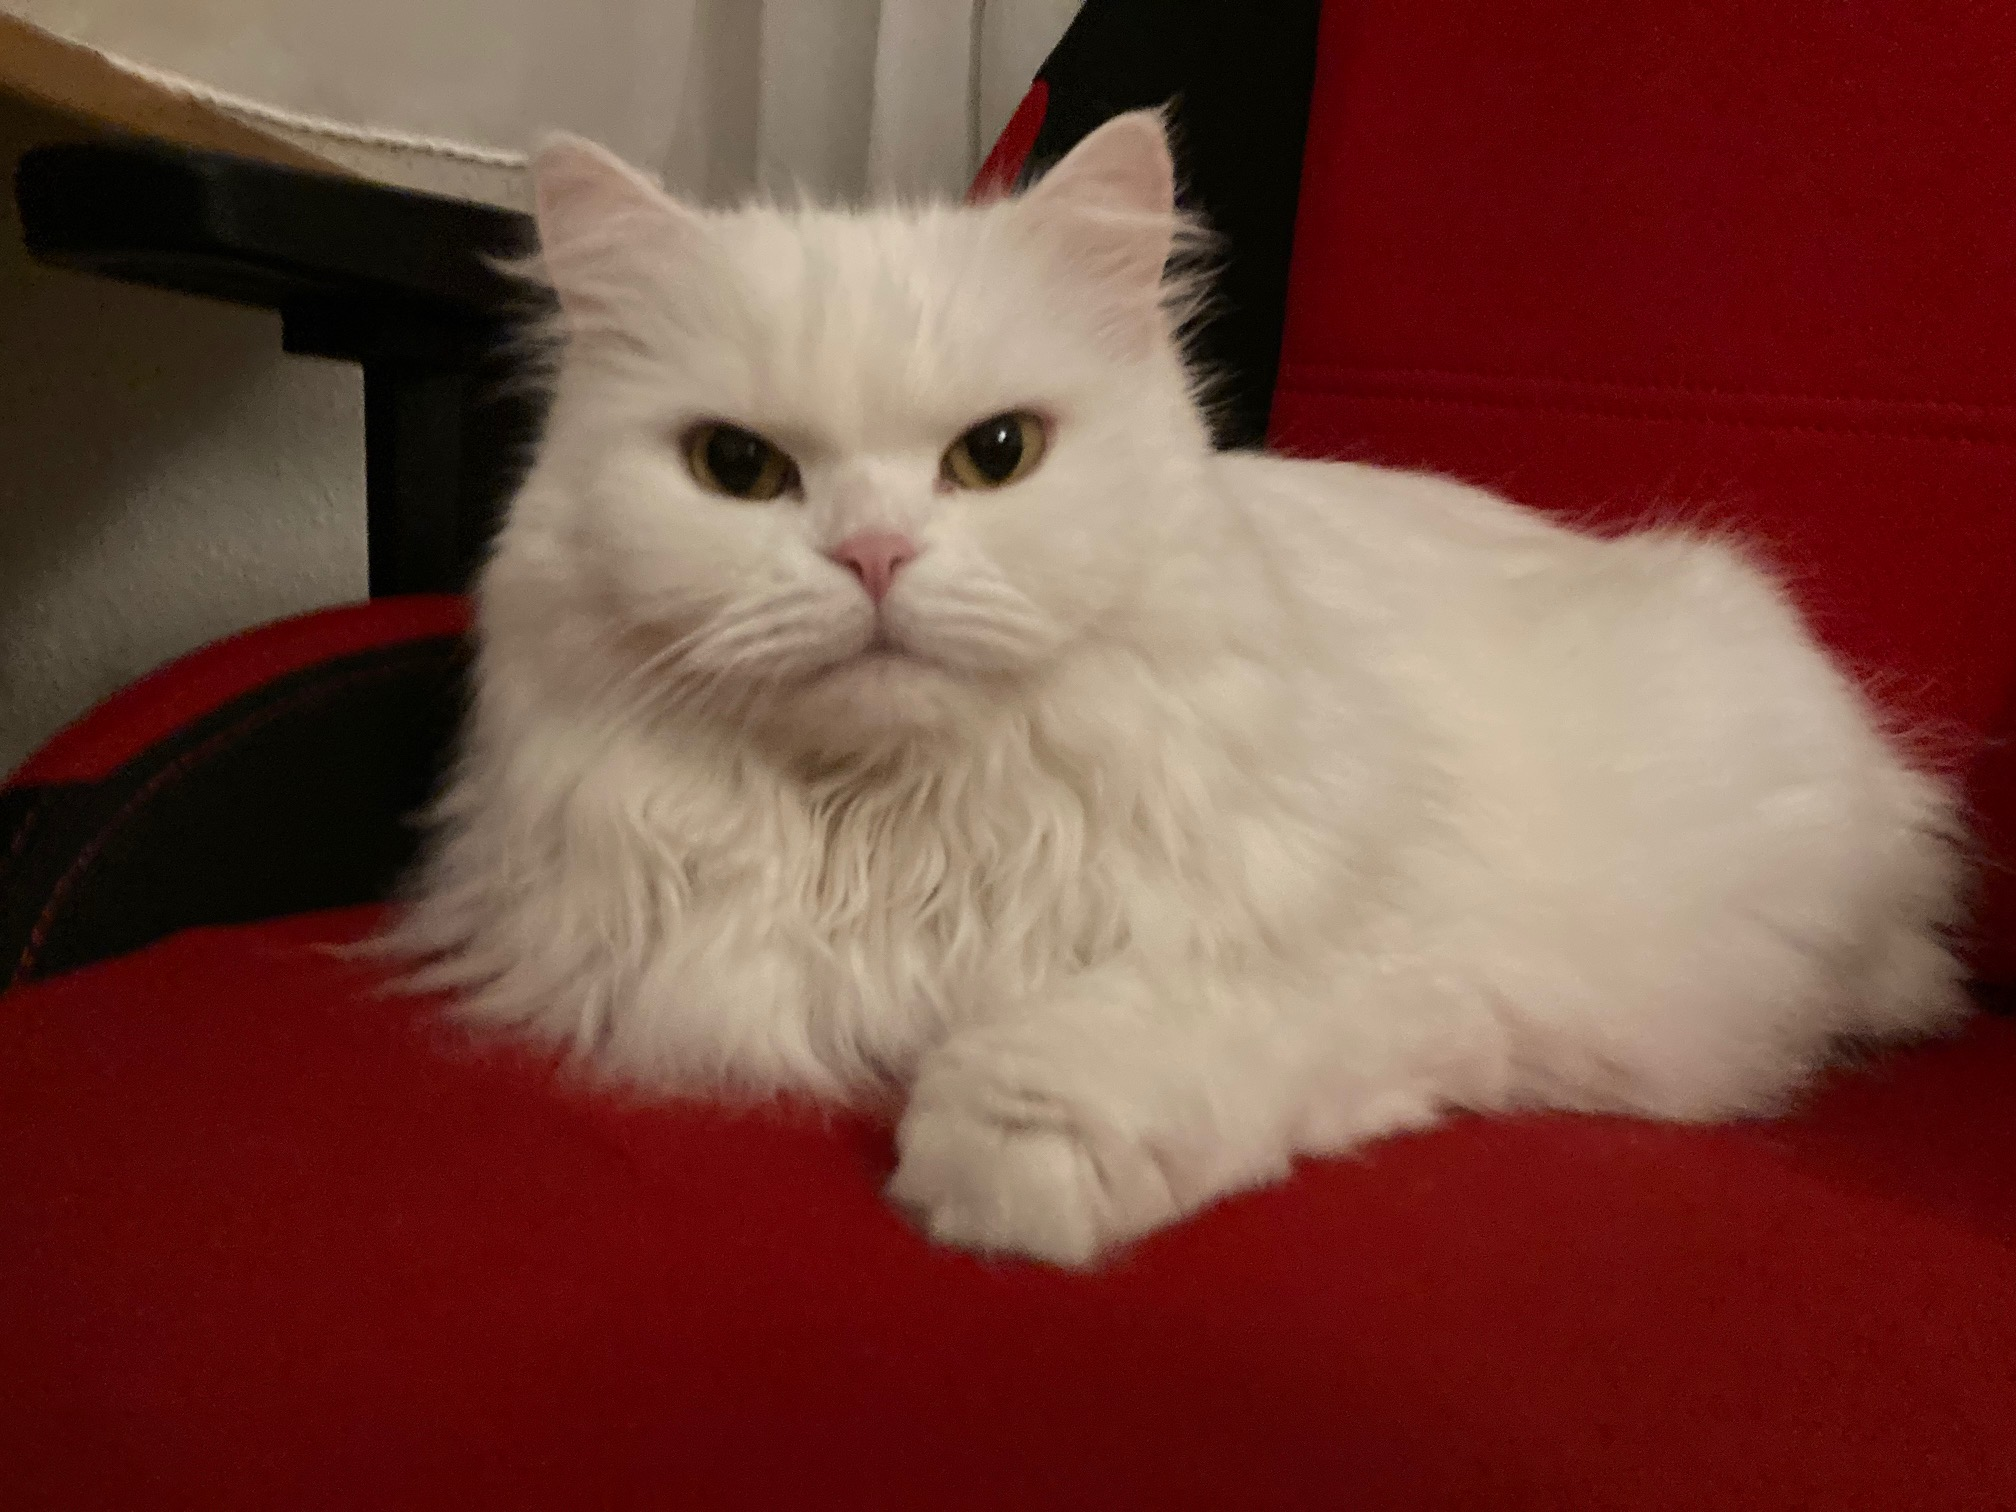
\includegraphics[width=0.49\textwidth]{Bilder/Katze} \\
\end{tabular}


\the\textwidth

\the\linewidth

\the\columnwidth

\begin{itemize}
	\item \the\textwidth
	\item \the\linewidth
	\item \the\columnwidth
\end{itemize}

%!TeX root=Hauptdokument.tex
\chapter{Einführung}

\blindtext[20]

\blindtext[20]

\blindtext[20]


%!TeX root=Hauptdokument.tex
\chapter{Hauptteil}

\blindtext[20]

\blindtext[20]

\blindtext[20]

%!TeX root=Hauptdokument.tex
\chapter{Fazit}

\blindtext[200]

\blindtext[200]

\blindtext[200]


\end{document}